\subsection[Insertion]{Tri par insertion}

\begin{frame}
\frametitle{Tri par insertion}
\framesubtitle{Idea}
\begin{itemize}
\item A chaque itération, prendre une élement dans la partie non triée du tableau et le mettre au bon endroit dans la partie triée
\item 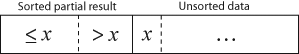
\includegraphics[width=0.5\textwidth]{./1-sorting/img/insertion_before}
\item deviens
\item 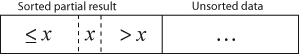
\includegraphics[width=0.5\textwidth]{./1-sorting/img/insertion_after}
\end{itemize}
\end{frame}

\begin{frame}
\frametitle{Tri par insertion}
\begin{table}
\begin{tabular}{| c | c | c | c | c | c | c | c |}
\hline
6 & 5 & 3 & 1 & 8 & 7 & 2 & 4 \\ 
\hline
\end{tabular}
\end{table}
\end{frame}

\begin{frame}
\frametitle{Tri par insertion}
\begin{table}
\begin{tabular}{| c | c | c | c | c | c | c | c |}
\hline
\cellcolor{red!25}6 & 5 & 3 & 1 & 8 & 7 & 2 & 4 \\ 
\hline
\end{tabular}
\end{table}
\begin{table}
\begin{tabular}{| c | c | c | c | c | c | c | c |}
\hline
\cellcolor{blue!25}6 & 5 & 3 & 1 & 8 & 7 & 2 & 4 \\ 
\hline
\end{tabular}
\end{table}
\end{frame}

\begin{frame}
\frametitle{Tri par insertion}
\begin{table}
\begin{tabular}{| c | c | c | c | c | c | c | c |}
\hline
\cellcolor{blue!25}6 & \cellcolor{red!25}5 & 3 & 1 & 8 & 7 & 2 & 4 \\ 
\hline
\end{tabular}
\end{table}
\begin{table}
\begin{tabular}{| c | c | c | c | c | c | c | c |}
\hline
\cellcolor{red!25}5 & \cellcolor{blue!25}6 & 3 & 1 & 8 & 7 & 2 & 4 \\ 
\hline
\end{tabular}
\end{table}
\begin{table}
\begin{tabular}{| c | c | c | c | c | c | c | c |}
\hline
\cellcolor{blue!25}5 & \cellcolor{blue!25}6 & 3 & 1 & 8 & 7 & 2 & 4 \\ 
\hline
\end{tabular}
\end{table}
\end{frame}

\begin{frame}
\frametitle{Tri par insertion}
\begin{table}
\begin{tabular}{| c | c | c | c | c | c | c | c |}
\hline
\cellcolor{blue!25}5 & \cellcolor{blue!25}6 & \cellcolor{red!25}3 & 1 & 8 & 7 & 2 & 4 \\ 
\hline
\end{tabular}
\end{table}
\begin{table}
\begin{tabular}{| c | c | c | c | c | c | c | c |}
\hline
\cellcolor{blue!25}5 & \cellcolor{red!25}3 & \cellcolor{blue!25}6 & 1 & 8 & 7 & 2 & 4 \\ 
\hline
\end{tabular}
\end{table}
\begin{table}
\begin{tabular}{| c | c | c | c | c | c | c | c |}
\hline
\cellcolor{red!25}3 & \cellcolor{blue!25}5 & \cellcolor{blue!25}6 & 1 & 8 & 7 & 2 & 4 \\ 
\hline
\end{tabular}
\end{table}
\begin{table}
\begin{tabular}{| c | c | c | c | c | c | c | c |}
\hline
\cellcolor{blue!25}3 & \cellcolor{blue!25}5 & \cellcolor{blue!25}6 & 1 & 8 & 7 & 2 & 4 \\ 
\hline
\end{tabular}
\end{table}
\end{frame}

\begin{frame}
\frametitle{Tri par insertion}
\begin{table}
\begin{tabular}{| c | c | c | c | c | c | c | c |}
\hline
\cellcolor{blue!25}3 & \cellcolor{blue!25}5 & \cellcolor{blue!25}6 & \cellcolor{red!25}1 & 8 & 7 & 2 & 4 \\ 
\hline
\end{tabular}
\end{table}
\begin{table}
\begin{tabular}{| c | c | c | c | c | c | c | c |}
\hline
\cellcolor{blue!25}3 & \cellcolor{blue!25}5 & \cellcolor{red!25}1 & \cellcolor{blue!25}6 & 8 & 7 & 2 & 4 \\ 
\hline
\end{tabular}
\end{table}
\begin{table}
\begin{tabular}{| c | c | c | c | c | c | c | c |}
\hline
\cellcolor{blue!25}3 & \cellcolor{red!25}1 & \cellcolor{blue!25}5 & \cellcolor{blue!25}6 & 8 & 7 & 2 & 4 \\ 
\hline
\end{tabular}
\end{table}
\begin{table}
\begin{tabular}{| c | c | c | c | c | c | c | c |}
\hline
\cellcolor{red!25}1 & \cellcolor{blue!25}3 & \cellcolor{blue!25}5 & \cellcolor{blue!25}6 & 8 & 7 & 2 & 4 \\ 
\hline
\end{tabular}
\end{table}
\begin{table}
\begin{tabular}{| c | c | c | c | c | c | c | c |}
\hline
\cellcolor{blue!25}1 & \cellcolor{blue!25}3 & \cellcolor{blue!25}5 & \cellcolor{blue!25}6 & 8 & 7 & 2 & 4 \\ 
\hline
\end{tabular}
\end{table}
\end{frame}

\begin{frame}
\frametitle{Tri par insertion}
\begin{table}
\begin{tabular}{| c | c | c | c | c | c | c | c |}
\hline
\cellcolor{blue!25}1 & \cellcolor{blue!25}3 & \cellcolor{blue!25}5 & \cellcolor{blue!25}6 & \cellcolor{red!25}8 & 7 & 2 & 4 \\ 
\hline
\end{tabular}
\end{table}
\begin{table}
\begin{tabular}{| c | c | c | c | c | c | c | c |}
\hline
\cellcolor{blue!25}1 & \cellcolor{blue!25}3 & \cellcolor{blue!25}5 & \cellcolor{blue!25}6 & \cellcolor{blue!25}8 & 7 & 2 & 4 \\ 
\hline
\end{tabular}
\end{table}
\end{frame}

\begin{frame}
\frametitle{Tri par insertion}
\begin{table}
\begin{tabular}{| c | c | c | c | c | c | c | c |}
\hline
\cellcolor{blue!25}1 & \cellcolor{blue!25}3 & \cellcolor{blue!25}5 & \cellcolor{blue!25}6 & \cellcolor{blue!25}8 & \cellcolor{red!25}7 & 2 & 4 \\ 
\hline
\end{tabular}
\end{table}
\begin{table}
\begin{tabular}{| c | c | c | c | c | c | c | c |}
\hline
\cellcolor{blue!25}1 & \cellcolor{blue!25}3 & \cellcolor{blue!25}5 & \cellcolor{blue!25}6 & \cellcolor{red!25}7 & \cellcolor{blue!25}8 & 2 & 4 \\ 
\hline
\end{tabular}
\end{table}
\begin{table}
\begin{tabular}{| c | c | c | c | c | c | c | c |}
\hline
\cellcolor{blue!25}1 & \cellcolor{blue!25}3 & \cellcolor{blue!25}5 & \cellcolor{blue!25}6 & \cellcolor{blue!25}7 & \cellcolor{blue!25}8 & 2 & 4 \\ 
\hline
\end{tabular}
\end{table}
\end{frame}

\begin{frame}
\frametitle{Tri par insertion}
\begin{table}
\begin{tabular}{| c | c | c | c | c | c | c | c |}
\hline
\cellcolor{blue!25}1 & \cellcolor{blue!25}3 & \cellcolor{blue!25}5 & \cellcolor{blue!25}6 & \cellcolor{blue!25}7 & \cellcolor{blue!25}8 & \cellcolor{red!25}2 & 4 \\ 
\hline
\end{tabular}
\end{table}
\begin{table}
\begin{tabular}{| c | c | c | c | c | c | c | c |}
\hline
\cellcolor{blue!25}1 & \cellcolor{blue!25}3 & \cellcolor{blue!25}5 & \cellcolor{blue!25}6 & \cellcolor{blue!25}7 & \cellcolor{red!25}2 & \cellcolor{blue!25}8 & 4 \\ 
\hline
\end{tabular}
\end{table}
\begin{table}
\begin{tabular}{| c | c | c | c | c | c | c | c |}
\hline
\cellcolor{blue!25}1 & \cellcolor{blue!25}3 & \cellcolor{blue!25}5 & \cellcolor{blue!25}6 & \cellcolor{red!25}2 & \cellcolor{blue!25}7 & \cellcolor{blue!25}8 & 4 \\ 
\hline
\end{tabular}
\end{table}
\begin{table}
\begin{tabular}{| c | c | c | c | c | c | c | c |}
\hline
\cellcolor{blue!25}1 & \cellcolor{blue!25}3 & \cellcolor{blue!25}5 & \cellcolor{red!25}2 & \cellcolor{blue!25}6 & \cellcolor{blue!25}7 & \cellcolor{blue!25}8 & 4 \\ 
\hline
\end{tabular}
\end{table}
\begin{table}
\begin{tabular}{| c | c | c | c | c | c | c | c |}
\hline
\cellcolor{blue!25}1 & \cellcolor{blue!25}3 & \cellcolor{red!25}2 & \cellcolor{blue!25}5 & \cellcolor{blue!25}6 & \cellcolor{blue!25}7 & \cellcolor{blue!25}8 & 4 \\ 
\hline
\end{tabular}
\end{table}
\begin{table}
\begin{tabular}{| c | c | c | c | c | c | c | c |}
\hline
\cellcolor{blue!25}1 & \cellcolor{red!25}2 & \cellcolor{blue!25}3 & \cellcolor{blue!25}5 & \cellcolor{blue!25}6 & \cellcolor{blue!25}7 & \cellcolor{blue!25}8 & 4 \\ 
\hline
\end{tabular}
\end{table}
\begin{table}
\begin{tabular}{| c | c | c | c | c | c | c | c |}
\hline
\cellcolor{blue!25}1 & \cellcolor{blue!25}2 & \cellcolor{blue!25}3 & \cellcolor{blue!25}5 & \cellcolor{blue!25}6 & \cellcolor{blue!25}7 & \cellcolor{blue!25}8 & 4 \\ 
\hline
\end{tabular}
\end{table}
\end{frame}

\begin{frame}
\frametitle{Tri par insertion}
\begin{table}
\begin{tabular}{| c | c | c | c | c | c | c | c |}
\hline
\cellcolor{blue!25}1 & \cellcolor{blue!25}2 & \cellcolor{blue!25}3 & \cellcolor{blue!25}5 & \cellcolor{blue!25}6 & \cellcolor{blue!25}7 & \cellcolor{blue!25}8 & \cellcolor{red!25}4 \\ 
\hline
\end{tabular}
\end{table}
\begin{table}
\begin{tabular}{| c | c | c | c | c | c | c | c |}
\hline
\cellcolor{blue!25}1 & \cellcolor{blue!25}2 & \cellcolor{blue!25}3 & \cellcolor{blue!25}5 & \cellcolor{blue!25}6 & \cellcolor{blue!25}7 & \cellcolor{red!25}4 & \cellcolor{blue!25}8 \\ 
\hline
\end{tabular}
\end{table}
\begin{table}
\begin{tabular}{| c | c | c | c | c | c | c | c |}
\hline
\cellcolor{blue!25}1 & \cellcolor{blue!25}2 & \cellcolor{blue!25}3 & \cellcolor{blue!25}5 & \cellcolor{blue!25}6 & \cellcolor{red!25}4 & \cellcolor{blue!25}7 & \cellcolor{blue!25}8 \\ 
\hline
\end{tabular}
\end{table}
\begin{table}
\begin{tabular}{| c | c | c | c | c | c | c | c |}
\hline
\cellcolor{blue!25}1 & \cellcolor{blue!25}2 & \cellcolor{blue!25}3 & \cellcolor{blue!25}5 & \cellcolor{red!25}4 & \cellcolor{blue!25}6 & \cellcolor{blue!25}7 & \cellcolor{blue!25}8 \\ 
\hline
\end{tabular}
\end{table}
\begin{table}
\begin{tabular}{| c | c | c | c | c | c | c | c |}
\hline
\cellcolor{blue!25}1 & \cellcolor{blue!25}2 & \cellcolor{blue!25}3 & \cellcolor{red!25}4 & \cellcolor{blue!25}5 & \cellcolor{blue!25}6 & \cellcolor{blue!25}7 & \cellcolor{blue!25}8 \\ 
\hline
\end{tabular}
\end{table}
\begin{table}
\begin{tabular}{| c | c | c | c | c | c | c | c |}
\hline
\cellcolor{blue!25}1 & \cellcolor{blue!25}2 & \cellcolor{blue!25}3 & \cellcolor{blue!25}4 & \cellcolor{blue!25}5 & \cellcolor{blue!25}6 & \cellcolor{blue!25}7 & \cellcolor{blue!25}8 \\ 
\hline
\end{tabular}
\end{table}
\end{frame}

\begin{frame}
\frametitle{Tri par insertion}
\framesubtitle{Complexité}
\begin{table}
\begin{tabular}{| c | c | c | c |}
\hline
Moyenne & Meilleure & Pire & Mémoire\\ 
\hline
O(n\textsuperscript{2}) & O(n) & O(n\textsuperscript{2}) & O(1)\\
\hline
\end{tabular}
\end{table}
\end{frame}